\chapter{Estudo de caso (QIE)}
\label{cap:estudo}
Neste capítulo será descrita a utilização do processo de alinhamento através de um estudo de caso, o QIE. O QIE foi escolhido, pois se trata de um projeto que pretende cruzar informações sobre a comunidade brasileira de informática na educação. Este capítulo está estruturado em três seções. A seção \ref{sec:estudo_descricao} apresenta uma descrição do estudo de caso e a conversão dos dados para RDF.

\section{Descrição do estudo}
\label{sec:estudo_descricao}
Para validar a eficácia da solução, foi solicitado a membros da comunidade de informática na educação que sugerissem perguntas de seu interesse. Como resultado foi levantado um conjunto contendo mais de 30 questões. A Tabela \ref{tab:questions} apresenta as questões propostas pelos membros.

\begin{table}[!ht]
	\centering
	\caption{Perguntas sugeridas pela comunidade}
	\label{tab:questions}
	\begin{tabular}{|l|l|}
		\hline
		ID  & Questões                                                                          \\ \hline
		Q01 & Quantos pesquisadores?                                                            \\ \hline
		Q02 & Quais pesquisadores?                                                              \\ \hline
		Q03 & Onde estão? (Estado)                                                              \\ \hline
		Q04 & Onde estão? (Universidade)                                                        \\ \hline
		Q05 & Quais são Doutores?                                                               \\ \hline
		Q06 & Quantos são Doutores?                                                             \\ \hline
		Q07 & Quem possui marca?                                                                \\ \hline
		Q08 & Onde fizemos os nossos doutorados?                                                \\ \hline
		Q09 & Onde fizemos os nossos pós-doutorados?                                            \\ \hline
		Q10 & Quantas publicações o autor “z” tem no evento “x”?                                \\ \hline
		Q11 & Quantos trabalhos foram publicados no evento “x”?                                 \\ \hline
		Q12 & Quantos autores publicaram no evento “x”?                                         \\ \hline
		Q13 & Quantos artigos foram publicados no periódico “y”?                                \\ \hline
		Q14 & Lista de Doutores + Email (RBIE)                                                  \\ \hline
		Q15 & Lista de Autores + Competência + Email                                            \\ \hline
		Q16 & Lista de Artigos publicados na RBIE - Geral                                       \\ \hline
		Q17 & Quantos são bolsistas e qual o nível? (DT/PQ)                                     \\ \hline
		Q18 & Quais são as principais competências da comunidade de IE?                         \\ \hline
		Q19 & Quais conceitos são explorados?                                                   \\ \hline
		Q20 & Quais os temas são mais pesquisados em IE?                                        \\ \hline
		Q21 & Quais pesquisadores colaboram entre si?                                           \\ \hline
		Q22 & Quais instituições colaboram entre si?                                            \\ \hline
		Q23 & Quais são os trabalhos relacionados?                                              \\ \hline
		Q24 & Como os conceitos explorados evoluem ao longo do tempo?                           \\ \hline
		Q25 & Mapa de tendências de pesquisa em uma linha do tempo.                             \\ \hline
		Q26 & O quão um pesquisador X está publicando no SBIE, WIE e RBIE ao longo do tempo?    \\ \hline
		Q27 & Lista de bolsistas de produtividade                                               \\ \hline
		Q28 & Quais as instituições?                                                            \\ \hline
		Q29 & Quais autores publicaram na conferência "X"?                                      \\ \hline
		Q30 & Quantos pesquisadores de IE estão em PPGs de CC?                                  \\ \hline
		Q31 & Quem são os maiores especialistas em recursos digitais e objetos de aprendizagem? \\ \hline
	\end{tabular}
\end{table}

De acordo com as perguntas realizadas, pode-se perceber que em alguns momentos é necessário o cruzamento de informações dos pesquisadores e suas publicações de diferentes fontes. , sendo elas a Revista Brasileira de Informática na Educação\footnote{\url{http://www.br-ie.org/pub/index.php/rbie}} (RBIE), Workshop de informática na Escola\footnote{\url{http://www.br-ie.org/pub/index.php/wie }} (WIE), Simpósio Brasileiro de Informática na Educação\footnote{\url{http://www.br-ie.org/pub/index.php/sbie}} (SBIE) e currículum Lattes\footnote{\url{http://lattes.cnpq.br}}. Vale a pena ressaltar que os \textit{datasets} foram disponibilizados como arquivos XML, sendo necessário transformá-los para RDF.

Para modelar os dados, foram utilizadas as ontologias dac\footnote{\url{https://github.com/josmarios/dac/blob/master/Ontologies/dacV2.1.owl}} e lattes\footnote{\url{https://github.com/armandobs14/lattes/blob/master/lattes.owl}}. A primeira tem o objetivo de modelar o domínio de publicação (ver Figura \ref{fig:dac}). A segunda foi construída para modelar o domínio do lattes (ver Figura \ref{fig:lattes}).

\begin{figure}[!ht]
	\centering
	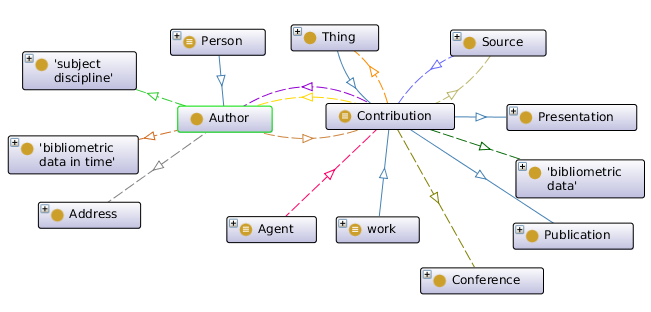
\includegraphics[width=0.9\textwidth]{./imagens/dac-mainview.png}
	\caption{Taxonomia da ontologia dac}
	\label{fig:dac}
\end{figure}

\begin{figure}[!ht]
	\centering
	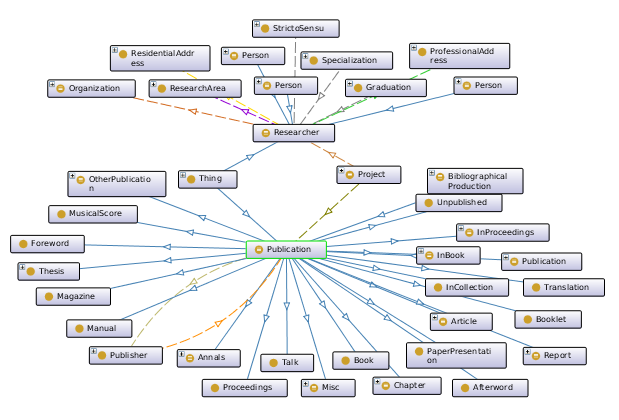
\includegraphics[width=0.9\textwidth]{./imagens/lattes-mainview.png}
	\caption{Taxonomia da ontologia lattes}
	\label{fig:lattes}
\end{figure}

Para transformar os dados para RDF foi utilizada a ferramenta OpenRefine\footnote{\url{http://openrefine.org}} com a extensão para suportar RDF. Essa ferramenta foi selecionada devido a sua facilidade para criar os templates de transformação. Após a transformação dos dados, as ontologias e os dados foram persistidos no Virtuoso\footnote{\url{https://virtuoso.openlinksw.com}}. A Figura \ref{fig:conversao} representa o processo de conversão dos dados.

\begin{figure}[!ht]
	\centering
	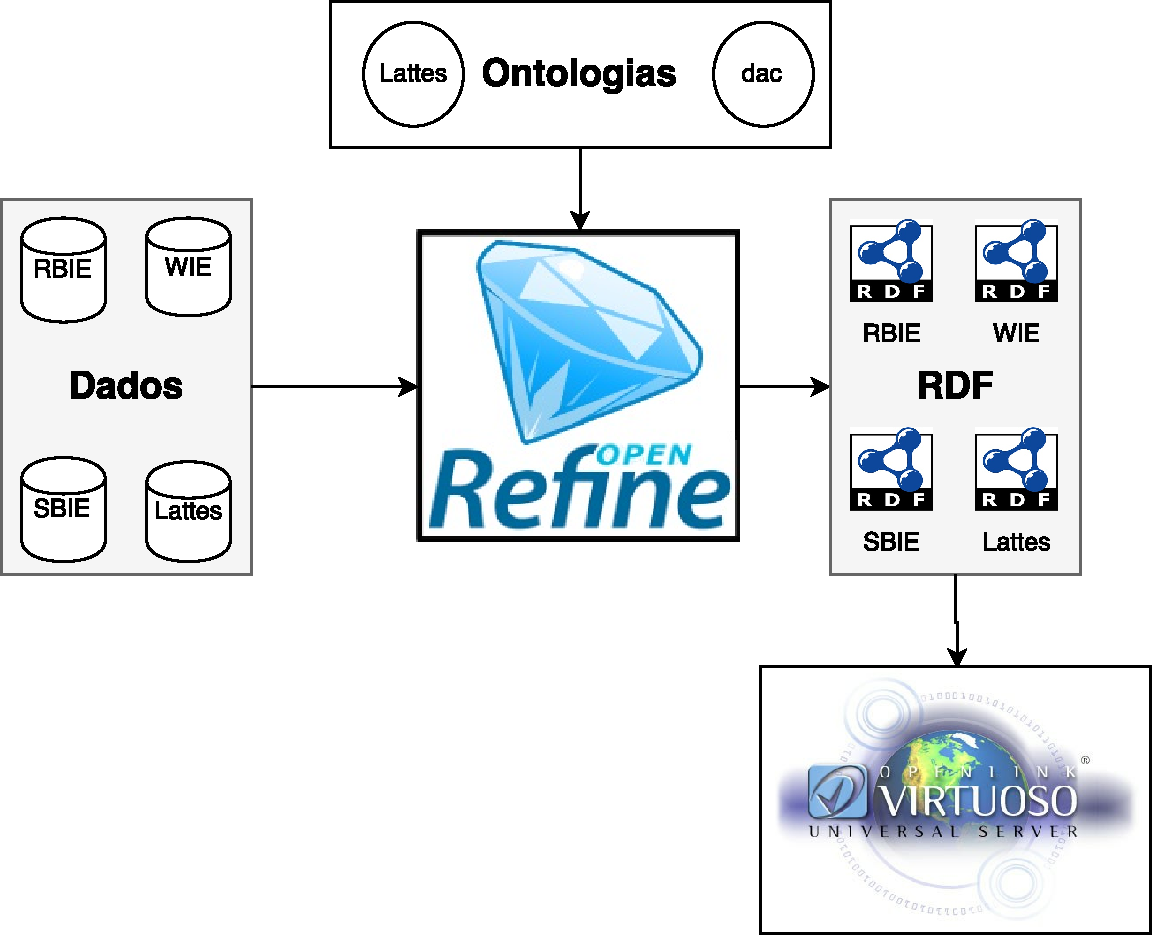
\includegraphics[width=0.9\textwidth]{./imagens/conversao.pdf}
	\caption{Processo de conversão para rdf}
	\label{fig:conversao}
\end{figure}

Com o processo de conversão dos dados foram geradas 1.1 Milhões de triplas. As triplas estão distribuídas da seguinte forma: (96\%, 1094307 triplas) pertencem ao Lattes, (1.61\%,18363 triplas) pertencem ao SBIE, (1.21\%, 14601 triplas) pertencem ao WIE e (1.1\%, 12503 triplas) pertencem ao RBIE.

\newpage
\section{Execução do processo}
Nesta seção pretende-se descrever como foi realizada cada uma das etapas do processo de correspondência. 

\subsection{Selecionar \textit{Datasets}}
\label{sub:selecionar_datasets}
\subsection{Identificar Conceitos}
\subsubsection{Conceito Principal}
\subsubsection{Conceito Relacionado}
\subsection{Listar Recursos}
\subsection{Alinhar Dados}
\subsubsection{Alinhamento Simples}
\subsubsection{Alinhamento em Cascata}

\section{Resultados}
